\begin{multicols}{2}

пропорциональность значения энергии квантовому числу n. Уровни энергии гармонического осциллятора расположены на равных расстояниях друг от друга. И это также отражает решение (6). Правда в строгом решении эти расстояния равны $h\nu$, а в нестрогом - $\frac{\pi}{4}h\nu$ (Опыт подтверждает, конечно, строгое решение.) Кроме того, согласно строгому решению минимальная энергия гармоничного осцилятора при n=0, отлична от нуля и равна $\frac{h\nu}{2}$ (рис 4а). В нестрогом решении $Е_0=0$ (рис 4б).\\
\indent Из условия квантования (6) следует, что возможные значения максимального отклонения от положения\columnbreak \\
$x_n$ и $x_{n+1}$, например, для шарика массы m = 10 г, колеблющегося на пружине жёсткости k=1000 н/м. И вы убедитесь, что это расстояние столь мало, что спектор возможных значений x практически непрерывный. И только для микрочастиц спектор $E_n$ и $x_n$ дискретны.
\subsection*{Атом водорода}
Рассмотри ещё одну задачу - о квантовыании энергии атома водорода. Впервые эта задача была решена Нильсом Бором. Он расчитал спектор атома водорода пользуясь так называемой планетарной моделью. Хотя расчётные значения энергии электрона совпадали с наблюдаемым спектром,

\end{multicols}

\begin{center}
    \begin{minipage}{0.45\textwidth}
        \centering
        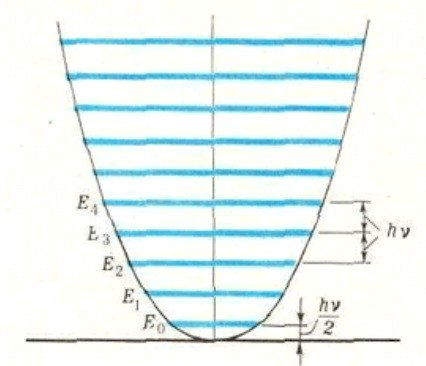
\includegraphics[width=0.8\textwidth]{график1.png} \\
        \small Рис. 4а.
    \end{minipage}
    \hfill
    \begin{minipage}{0.45\textwidth}
        \centering
        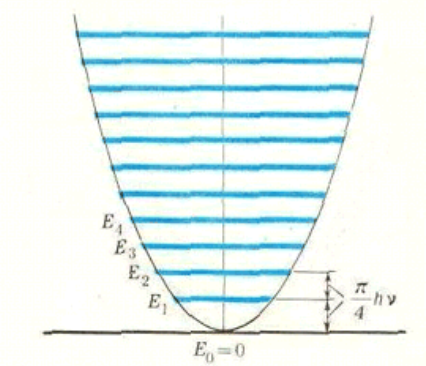
\includegraphics[width=0.8\textwidth]{график2.png} \\
        \small Рис. 4б.
    \end{minipage}
\end{center}

\begin{multicols}{2}
равновесия дискретны:\\
{\large $E_n=\frac{kx_n^2}{2}=\frac{\pi}{4}nh\nu$\\}
откуда\\
{\large $x_n=\sqrt{\frac{\pi}{2}nh\frac{\nu}{k}}$}  \indent (8)\\
Этот вывод кажется совсем странным, ведь амплитуда колебаний, по существу, задаётся начальным смещением из положения равновесия. А из "житейского" опыта известно, что смещение, скажем, шарика на пружинке можно менять плавно, непрерывно. В чём же дело? Попробуйти сами, пользуясь формулой (8) найти расстояние между соседними значениями\columnbreak \\
Эта модель не позволяла расчитать другие характеристики атома.\\
\indent Согласно современным представлениям квантовой механики планетарная модель лишь очень условно отражает действительное поведение электронов. В атоме водорода единственный электрон какбы образует вокруг ядра электронное облако - облако отрицательного заряда, плотность которого характеризует велечинность нахождения электрона в данной области внутри атома. В невозбуждённом состоянии радиус сферы наибольшей плотности равен приблизительно 0,53 А. (В планитарной модели этому растоянию
\end{multicols}
